\section{Electric}

Kolejnym programem do projektowania schematów układów scalonych jest Electric,
opracowany przez S. M. Rubina w 1981 roku.
Od samego początku posiadał otwarty kod źródłowy
oraz był udostępniany wielu uczelniom na całym świecie.
Oryginalnie napisany w języku C,
natomiast w 2003 rozpoczęto proces tłumaczenia na język Java, zakończony sukcesem w 2005 roku~\cite{electric_gnu}.
Dzięki temu program jest dostępny na każdy system,
na którym zainstalowana jest Java w wersji 1.6 lub więcej.
Do samej instalacji wystarczy natomiast pobrać plik \texttt{.jar} z oficjalnej strony programu~\cite{electric_sfs}.
Podobnie jak Microwind, Electric jest oprogramowaniem EDA, zawierający wiele modułów wspierających projektowanie układów scalonych.
Większość nich jest pod postacią dodatkowo instalowanych wtyczek,
poszerzających jego funkcjonalność~\cite{electric_sfs, electric_gnu}.\\
\indent Electric charakteryzuje się całkowicie odmienną metodą projektowania topografii niż większość programów.
Podobnie do edytorów schematów elektrycznych, używa podejścia połączeniowego,
w przeciwieństwie do reszty, gdzie występuje podejście geometryczne, czyli rysowanie prostokątów.
Oparcie projektowania o metodę połączeń polega na wstawianiu konkretnych elementów będących węzłami,
a następnie łączenie ich ze sobą.
Na przykład tranzystor jest już gotowym elementem, który można wstawić na schemat,
którego nie trzeba specjalnie rysować, jak to jest w przypadku programów Magic czy Microwind.
Upraszcza to cały proces projektowania,
natomiast problem może stanowić tworzenie układów o bardziej skomplikowanej i złożonej geometrii.\\
\indent Dzięki wykorzystaniu Javy, Electric posiada nowocześniejszy interfejs graficzny,
pokazany na rys.~\ref{fig:electric_okno}.
Także sposób poruszania się po obszarze oraz skróty klawiszowe są bardziej zgodne z obecnymi standardami,
dzięki czemu program jest bardziej intuicyjny w obsłudze.

\begin{figure}[h]
    \centering
    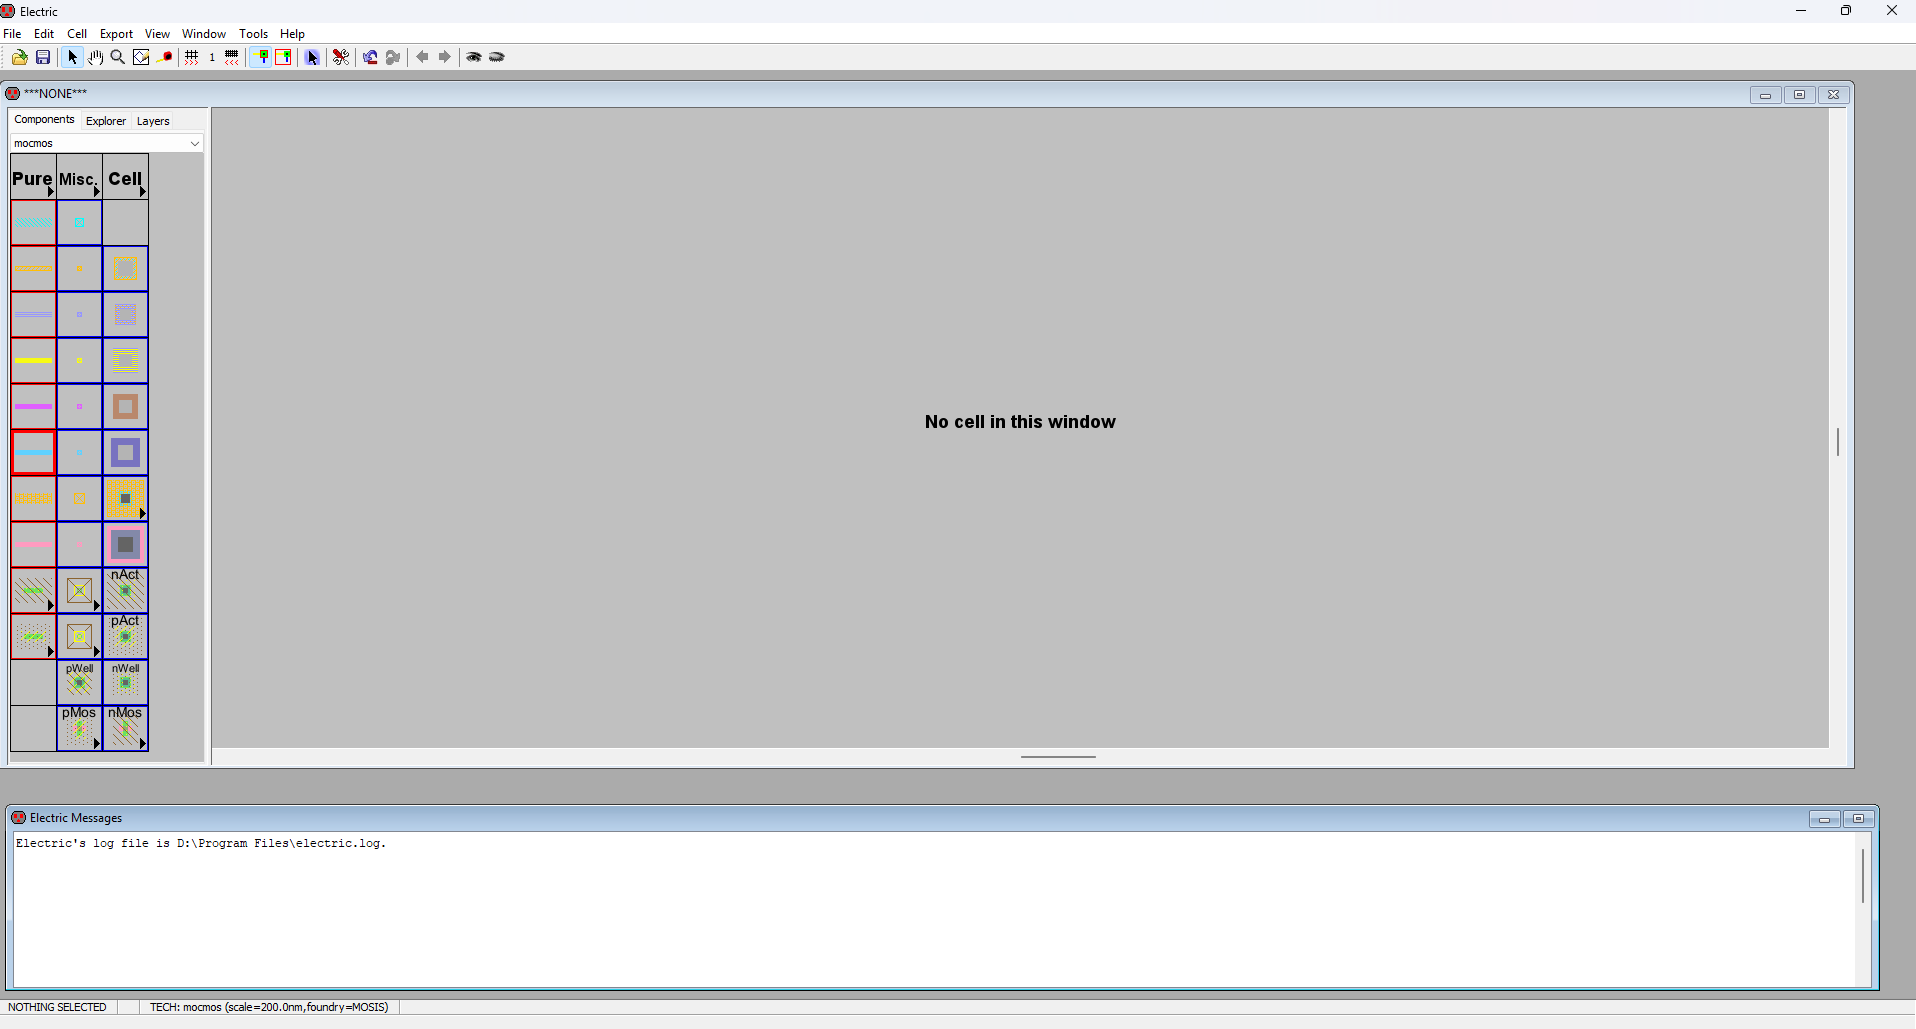
\includegraphics[width=.9\textwidth]{chapters/chapter2/img/electric_okno}
    \caption[Widok głównego okna programu Electric.]{Widok głównego okna programu Electric, źródło:~\cite{electric_sfs}.}
    \label{fig:electric_okno}
\end{figure}

Prócz stałych pasków narzędzi i menu, program opiera się na pływających oknach,
dzięki czemu można jednocześnie mieć wyświetlone kilka narzędzi jednocześnie.
Na rys.~\ref{fig:electric_okno} przedstawiono okno do edycji schematu oraz okno dziennika zdarzeń.
Edytor zamiast palety warstw posiada okno z dostępnymi elementami, połączeniami i kontaktami pomiędzy warstwami.
W przypadku Electrica, do przedstawiania warstw wykorzystuje się jednolite kolory, oraz wzory,
co przedstawiono na rys.~\ref{fig:electric_tran}.
Przy edycji oraz rysowaniu topografii można zauważyć miganie elementów,
co wskazuje, że cały widok jest na nowo renderowany po każdej edycji lub przesunięciu.

\begin{figure}[h]
    \centering
    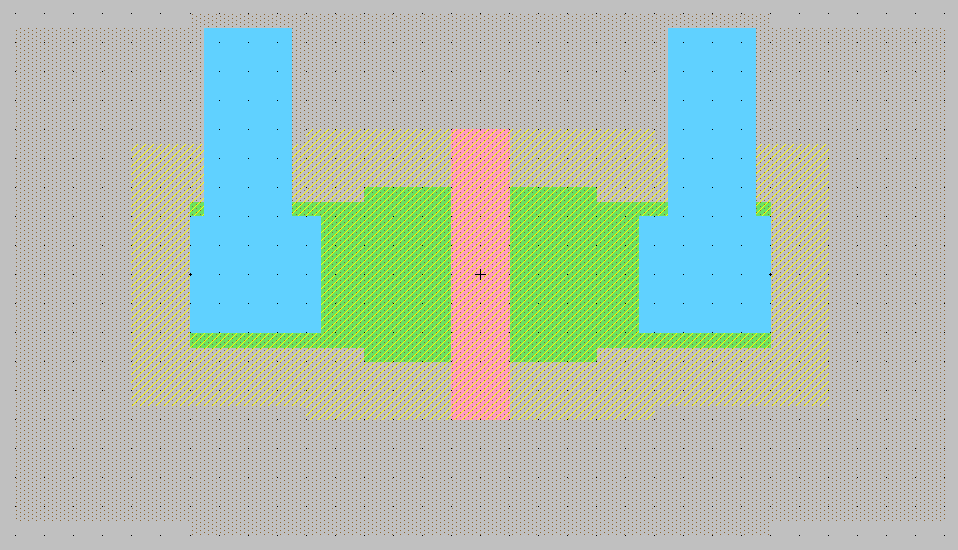
\includegraphics[width=.9\textwidth]{chapters/chapter2/img/electric_tran}
    \caption[Przykład tranzystora pMOS narysowanego w programie Electric]
    {
        Przykład tranzystora pMOS narysowanego w programie Electric,
        źródło: opracowanie własne.
    }
    \label{fig:electric_tran}
\end{figure}
